\section*{Backup}

%%%%%%%%%%%%%%%%%%%%%%%%%%%%%%%%%%%%%%%%%%%%%%%%%%%%%%%%%%%%%%%%%%%%%%%%%%%%
\begin{frame}[noframenumbering]{}
    \vfill
    \centering
    \begin{beamercolorbox}[sep=8pt,center,shadow=true,rounded=true]{title}
        \usebeamerfont{section title}\NoHyper\insertsection\par\endNoHyper
    \end{beamercolorbox}
    \vfill
\end{frame}
%%%%%%%%%%%%%%%%%%%%%%%%%%%%%%%%%%%%%%%%%%%%%%%%%%%%%%%%%%%%%%%%%%%%%%%%%%%%
\begin{frame}[noframenumbering]{Tag Propagation Register}
    \begin{table}[!t]
        \centering
        \caption{Tag Propagation Register configuration}
        \label{tab:tpr}
        \resizebox{\linewidth}{!}{%
            \setlength{\tabcolsep}{2pt}
            \begin{tabular}{@{}lcccccccc@{}}
                \toprule
                          & Load/Store Enable & Load/Store Mode & Logical Mode & Comparison Mode & Shift Mode & Jump Mode & Branch Mode & Arith Mode \\ \cmidrule(lr){2-2}\cmidrule(lr){3-3}\cmidrule(lr){4-4}\cmidrule(lr){5-5}\cmidrule(lr){6-6}\cmidrule(lr){7-7}\cmidrule(lr){8-8}\cmidrule(lr){9-9}
                Bit index & 17 16 15          & 13 12           & 11 10        & 9 8             & 7 6        & 5 4       & 3 2         & 1 0        \\ \midrule
                Policy V1 & 0 0 1             & 1  0            & 1  0         & 0 0             & 1 0        & 1 0       & 0 0         & 1 0        \\
                Policy V2 & 1 1 1             & 1  0            & 1  0         & 1 0             & 1 0        & 1 0       & 1 0         & 1 0        \\ \bottomrule
            \end{tabular}
        }
    \end{table}

    \begin{itemize}
        \justifying
        \item A Mode field for each class of instructions which specifies how to propagate the tags of the input operands to the output operand tag.
              \begin{itemize}
                  \justifying
                  \item the output tag keeps its old value (00);
                  \item the output tag is set to one, if both the input tags are set to one (01);
                  \item the output tag is set to one, if at least one input tag is set to one (10);
                  \item the output tag is set to zero (11).
              \end{itemize}
        \item The three bits in the L/S enable field allow the policy to enable the source, source-address, and destination-address tags, respectively
    \end{itemize}
\end{frame}

\begin{frame}[noframenumbering]{Tag Check Register}
    \begin{table}[!t]
        \centering
        \caption{Tag Check Register configuration}
        \label{tab:tcr}
        \resizebox{\linewidth}{!}{%
            \setlength{\tabcolsep}{2pt}
            \begin{tabular}{@{}lcccccccc@{}}
                \toprule
                          & Execute Check & Load/Store Check & Logical Check & Comparison Check & Shift Check & Jump Check & Branch Check & Arith Check \\\cmidrule(lr){2-2}\cmidrule(lr){3-3}\cmidrule(lr){4-4}\cmidrule(lr){5-5}\cmidrule(lr){6-6}\cmidrule(lr){7-7}\cmidrule(lr){8-8}\cmidrule(lr){9-9}
                Bit index & 21            & 20 19 18 17      & 16 15 14      & 13 12 11         & 10 9 8      & 7 6 5      & 4 3          & 2 1 0       \\ \midrule
                Policy V1 & 1             & 1 0 1 0          & 0 0 0         & 0 0 0            & 0 0 0       & 0 0 0      & 0 0          & 0 0 0       \\
                Policy V2 & 0             & 0 0 0 0          & 0 0 0         & 0 0 0            & 0 0 0       & 0 0 0      & 0 0          & 0 1 1       \\ \bottomrule
            \end{tabular}
        }
    \end{table}

    \begin{itemize}
        \justifying
        \item The tag-check rules restrict the operations that may be performed on tagged data. If the check bit for an operand tag is set to one and the corresponding tag is equal to one, an exception is raised.
              \begin{itemize}
                  \justifying
                  \item For all the classes except Load/Store, there are three tags to consider: first input, second input, and output tags
                  \item For the Load/Store class there are four tags to take into account: source-address, source, destination-address, and destination tags
                  \item the additional Execute Check field is associated with the program counter and specifies whether to raise a security exception when the program-counter tag is set to one
              \end{itemize}
    \end{itemize}
\end{frame}
%%%%%%%%%%%%%%%%%%%%%%%%%%%%%%%%%%%%%%%%%%%%%%%%%%%%%%%%%%%%%%%%%%%%%%%%%%%%
\begin{frame}[fragile,noframenumbering]{Case 2: WU-FTPd}
    \begin{itemize}
        \justifying
        \item The vulnerability is the use of an unchecked user input as the format string parameter in functions that perform formatting, e.g. printf()
        \item An attacker can use the format tokens, to write into arbitrary locations of memory, e.g. the return address of the function.
    \end{itemize}

    \centering
    \begin{minipage}[c]{\textwidth}
        \begin{lstlisting}[language=C,label=code:printfNFormat]
void echo(){
    int a;
    register int i asm("x8");
    a = i;
    printf("%224u%n%35u%n%253u%n%n", 1, (int*) (a-4), 1, (int*) (a-3), 1, (int*) (a-2), (int*) (a-1));
}\end{lstlisting}
    \end{minipage}
\end{frame}

\begin{frame}[noframenumbering]{}
    \begin{figure}
        \centering
        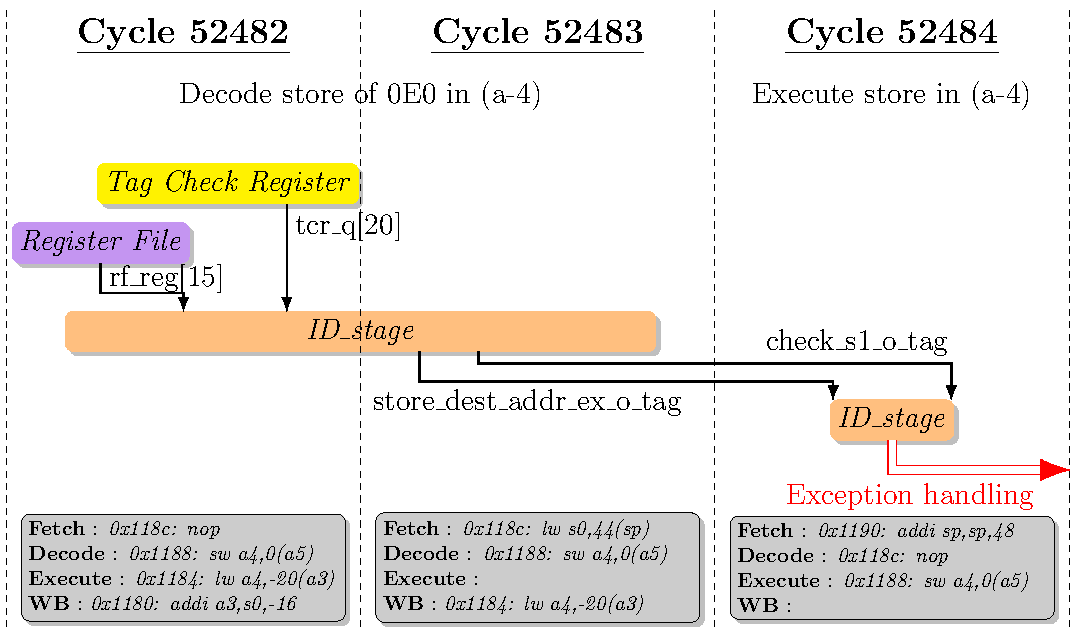
\includegraphics[height=.85\textheight]{src/2_vuln_assessment/img/wuftpd/ftpd_short.pdf}
        \caption{Temporal analysis of the tags propagation in a \textit{format string} attack}
        \label{fig:analyseTempoFormatString}
    \end{figure}
\end{frame}

\begin{frame}[noframenumbering]{}
    \begin{figure}
        \centering
        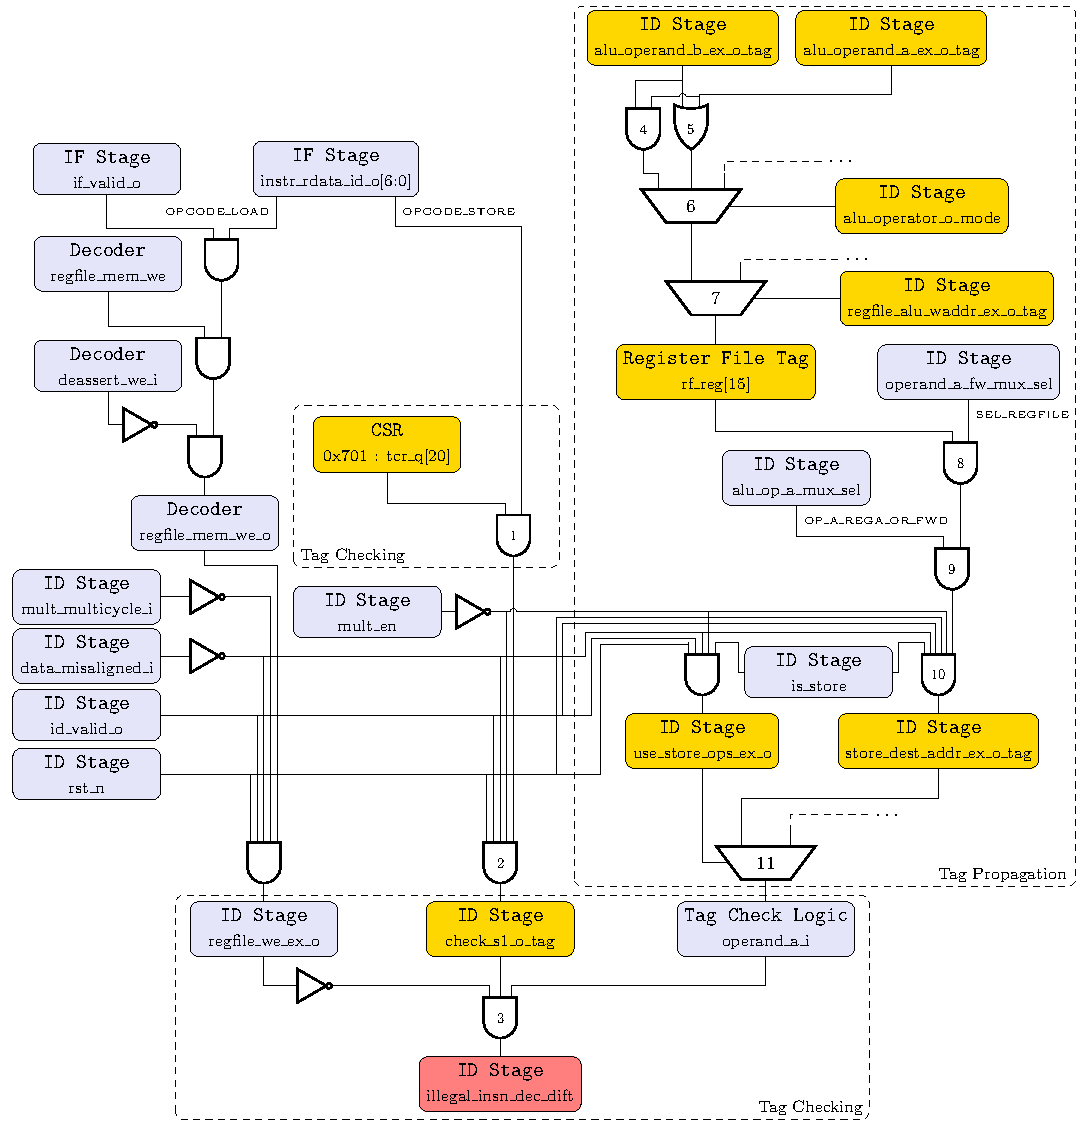
\includegraphics[height=.85\textheight]{src/2_vuln_assessment/img/wuftpd/arborescence_wuftpd.pdf}
        \caption{Logical analysis of the tags propagation in a \textit{format string} attack}
        \label{fig:analyseLogiqueFormatString}
    \end{figure}
\end{frame}
%%%%%%%%%%%%%%%%%%%%%%%%%%%%%%%%%%%%%%%%%%%%%%%%%%%%%%%%%%%%%%%%%%%%%%%%%%%%%%%%%%%%%%%%%%%%%%%%%%%%%%%%%%%%
\begin{frame}[fragile,noframenumbering]{Case 3: Compare/Compute}
    \begin{itemize}
        \justifying
        \item No software vulnerability
        \item Used to cover the DIFT surface
    \end{itemize}

    \centering
    \begin{minipage}[c]{\textwidth}
        \begin{lstlisting}[language=C,label=code:compareCompute]
int main(){
    int a, b = 5, c;
    register int reg asm("x9");
    a = reg;
    asm volatile("csrw 0x700, tprValue");
    asm volatile("csrw 0x701, tcrValue");
    asm volatile("p.spsw x0, 0(\%0);" :: "r" (&a));
    c = (a > b) ? (a-b) : (a+b);
        //42c:   ble a4,a5,448
        //430:   addi a5,s0,-16
        //434:   lw a4,-12(a5)
        //438:   addi a3,s0,-16
        //43c:   lw a5,-4(a3)
        //440:   sub a5,a4,a5
        //444:   j 45c
        //448:   addi a5,s0,-16
        //44c:   lw a4,-12(a5)
        //450:   addi a3,s0,-16
        //454:   lw a5,-4(a3)
        //458:   add a5,a4,a5
        //45c:   sw a5,-24(s0)
    return EXIT_SUCCESS;
}\end{lstlisting}
    \end{minipage}
\end{frame}

\begin{frame}[noframenumbering]{}
    \begin{figure}
        \centering
        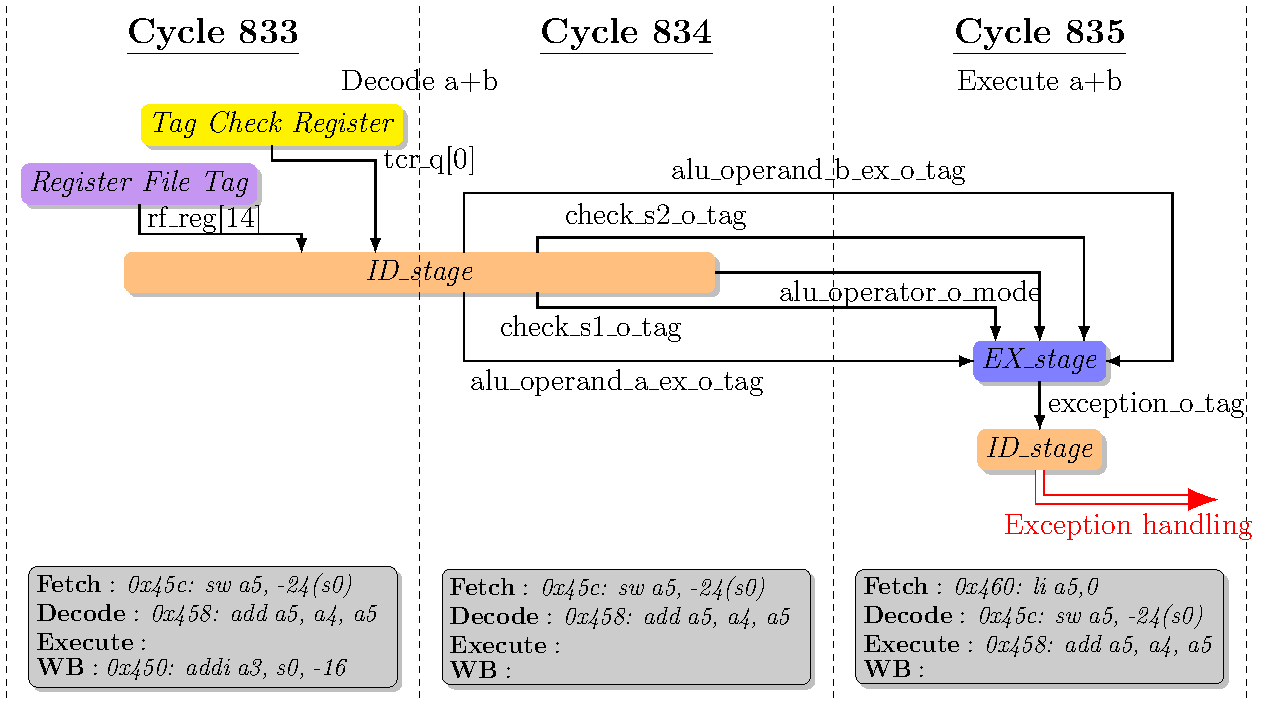
\includegraphics[height=.85\textheight]{src/2_vuln_assessment/img/comp_compu/attaquePropag_v3_short.pdf}
        \caption{Temporal analysis of the tags propagation in a \textit{format string} attack}
        \label{fig:analyseTempoCompCompute}
    \end{figure}
\end{frame}

\begin{frame}[noframenumbering]{}
    \begin{figure}
        \centering
        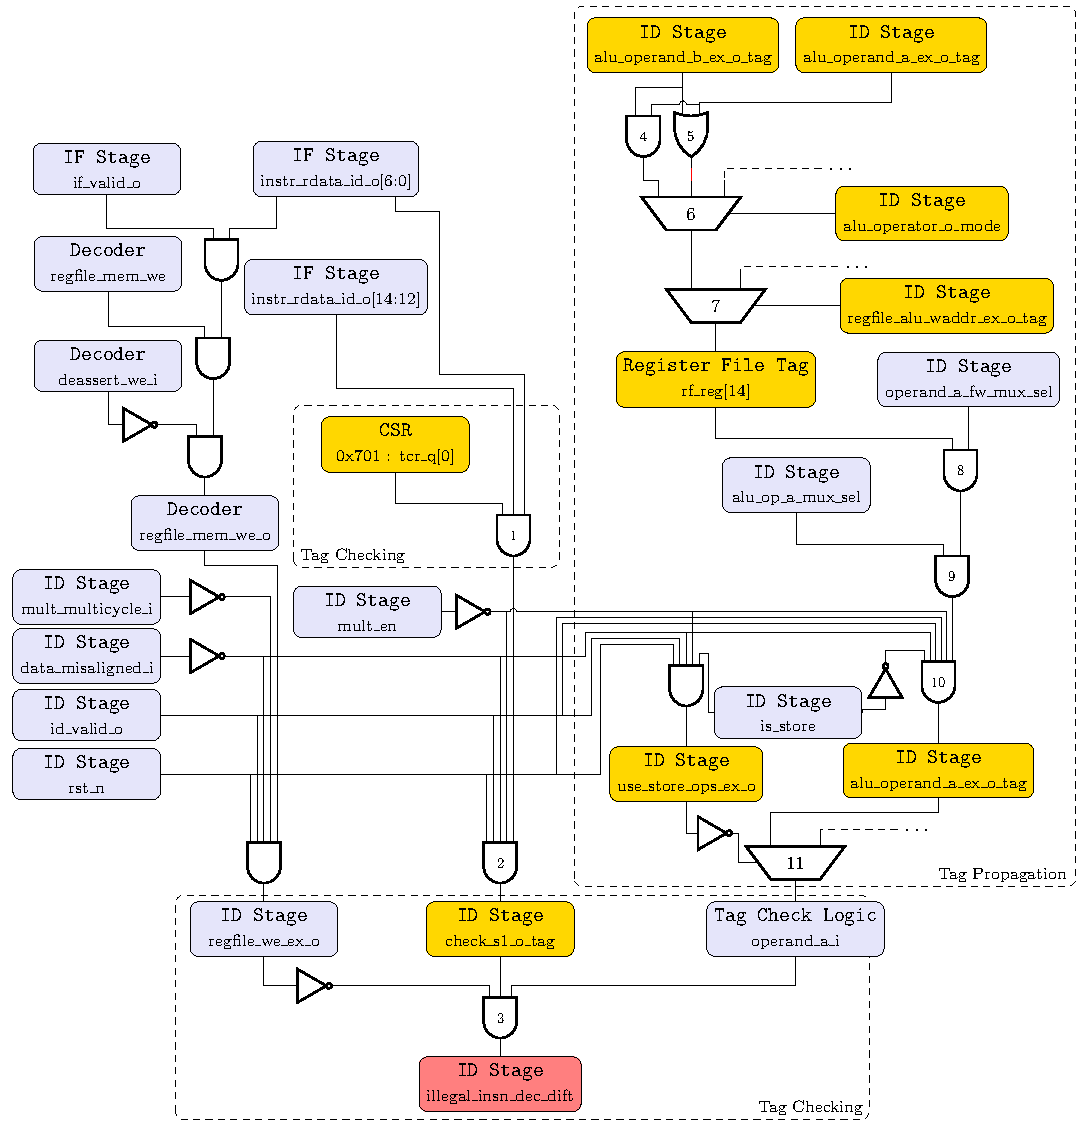
\includegraphics[height=.85\textheight]{src/2_vuln_assessment/img/comp_compu/arborescence_propagation.pdf}
        \caption{Logical analysis of the tags propagation in a \textit{format string} attack}
        \label{fig:analyseLogiqueCompCompute}
    \end{figure}
\end{frame}
%%%%%%%%%%%%%%%%%%%%%%%%%%%%%%%%%%%%%%%%%%%%%%%%%%%%%%%%%%%%%%%%%%%%%%%%%%%%%%%%%%%%%%%%%%%%%%%%%%%%%%%%%%%%